\documentclass[laboratorio]{guia}

\def \practnum {6} 
\def \practica {Circuito RLC}
% \def \practica {Circuito RLC: resonancia en serie y en paralelo}

\def \materia {Laboratorio de F\'\i sica II para Qu\'\i micos}
\def \periodo {2do. Cuatrimestre de 2015}
\def \catedra {Pablo Cobelli}
\def \website {http://materias.df.uba.ar/f2qa2015c2}
 
\usepackage{graphics}
\usepackage{amsmath}
\usepackage{amsfonts}
\usepackage{graphicx}
\usepackage{float}
\usepackage{wrapfig}
\usepackage{subfigure}
\usepackage{bm}
\usepackage{grffile}
\usepackage{color}
\usepackage{framed}
\usepackage[utf8]{inputenc}
\usepackage[T1]{fontenc}
\usepackage{lmodern}
\usepackage{circuitikz}
\usepackage[spanish]{babel}
\usepackage{babelbib}
\selectbiblanguage{spanish}

 

%----------------------------------------------------------
% Agrega al path de figuras el subdirectorio con el mismo
%     nombre que el archivo principal del proyecto
\graphicspath{{./\jobname/}}

%----------------------------------------------------------
% Definicion del entorno 'sabermas'
\makeatletter
\definecolor{shadecolor}{rgb}{0.89,0.91,0.94}
\newenvironment{sabermas}[1]{%
\vfill
\begin{shaded}
  \begin{center}
  {\textsection{Para saber m\'as}}
  \end{center}
  #1
\sf } 
{%
\end{shaded}%
}
\makeatother

%----------------------------------------------------------
% Definicion del entorno 'problema'
\newcounter{ContadorProblema}
\setcounter{ContadorProblema}{0}
\newcounter{TieneFiguraAsociada}
\setcounter{TieneFiguraAsociada}{0}
\newcounter{UbicacionFigura}
\setcounter{UbicacionFigura}{0}

\newenvironment{problema}[2][]
{%
    \ifx\relax#1\relax%
        \setcounter{TieneFiguraAsociada}{0}
        \else
        \setcounter{TieneFiguraAsociada}{1}
    \fi
    \def \archivofigura {#1}
    % 
    \refstepcounter{ContadorProblema}
    \noindent%
    \ifnum\value{TieneFiguraAsociada} < 1%
        {\sffamily \bfseries Problema \arabic{ContadorProblema}.}
        %{\sc {#1}}%
        \par\nobreak\par\nobreak%
        \medskip 
    \else
        % Va con figura; resta determinar de que lado.
        \ifnum\value{UbicacionFigura} < 1
            % Poner la figura del lado derecho
            \begin{minipage}{12.25cm}
            {\sffamily \bfseries Problema \arabic{ContadorProblema}.}
            %{\sc {#1}}%
            \par\nobreak\par\nobreak%
            \medskip 
        \else
            % Poner la figura del lado izquierdo
            \begin{minipage}{4.5cm}
                \centering
                \includegraphics[width=4.5cm]{\archivofigura}
                {\footnotesize {\sffamily Esquema asociado al 
                problema \arabic{ContadorProblema}}.}
            \end{minipage}\hfill%
            \begin{minipage}{12.25cm}
                {\sffamily \bfseries Problema \arabic{ContadorProblema}.}
                %{\sc {#1}}%
                \par\nobreak\par\nobreak%
                \medskip 
        \fi
    \fi
}
{%
    \ifnum\value{TieneFiguraAsociada} < 1%
        % \par \bigskip \vskip 0.3cm
    \else
        % Va con figura; resta determinar de que lado.
        \ifnum\value{UbicacionFigura} < 1
            % Poner la figura del lado derecho
            \end{minipage}\hfill%
            \begin{minipage}{4.5cm}
                \centering
                \includegraphics[width=4.5cm]{\archivofigura}
                {\footnotesize {\sffamily Esquema asociado al 
                problema \arabic{ContadorProblema}}.}
            \end{minipage}
        \else
            % Poner la figura del lado izquierdo
            \end{minipage}%
        \fi
    \fi
    \setcounter{TieneFiguraAsociada}{0}
    \par \bigskip \vskip 0.3cm
    % Permutamos el valor de la ubicacion
    \ifnum\value{UbicacionFigura} < 1
        \setcounter{UbicacionFigura}{1}
    \else
        \setcounter{UbicacionFigura}{0}
    \fi
}

%----------------------------------------------------------
% Definicion/Redefinicion de estilos
\renewcommand{\vec}[1]{\ensuremath{\mathbf{#1}}}



\hyphenation{ coe-fi-cien-tes coe-fi-cien-te au-to-va-lor
              au-to-va-lo-res co-rres-pon-der pro-ble-ma 
              cual-quie-ra po-la-ri-za-cio-nes }

\graphicspath{{./rlc/}}

\begin{document} 
\objetivo{
  Determinar experimentalmente la frecuencia de resonancia en un circuito RLC serie y paralelo.
  Estudiar además el desfasaje entre la diferencia de potencial y la corriente en función de la frecuencia de operación del circuito.   
  \tematicas{Circuitos de corrientes variables en el tiempo, RLC, resonancia.}
} 
\maketitle


\section{Circuito RLC serie}

\subsection{Introducci\'on}

Considere el circuito RLC mostrado en la figura \ref{fig:circuitoRLCserie}, en el cual un capacitor $C$, una inductancia $L$ y una resistencia $R$, se encuentran conectados en serie a un generador de funciones $G$.

\begin{figure}[hbt!]
    \centering
    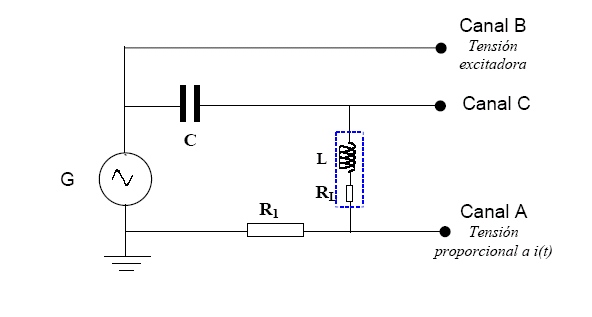
\includegraphics[width=9cm]{LG06--000.png}
    \caption{Esquema del circuito RLC serie.}
    \label{fig:circuitoRLCserie}
\end{figure}

Aplicando las leyes de Kirchhoff al circuito de la figura, tenemos:
\begin{equation}
    \varepsilon_G = \Delta V_L + \Delta V_R + \Delta V_C = L \dv{I}{t} + RI + \frac{q}{C},
\end{equation}
ecuación que podemos derivar nuevamente para obtener
\begin{equation}
    \dv{\varepsilon_G}{t} = L \dv[2]{I}{t} + R \dv{I}{t} + \frac{I}{C}.
\end{equation}

Si la fuerza eletromotriz suministrada por el generador es sinusoidal, entonces el término a la izquierda de la última ecuación es
\begin{equation}
    \varepsilon_G(t) = \Delta V_m \sen \left( \omega t \right),
\end{equation}
y la corriente circulante por el circuito estar\'a dada por
\begin{equation}
    I(t) = I_m \sen \left( \omega t + \Delta \phi \right),
\end{equation}
siendo $\omega = 2\pi f$ la frecuencia angular, y $f$ la frecuencia (medida en Hz) suministrada por el generador de funciones. 

La impedancia $Z$ del circuito es 
\begin{equation}
    Z = Z_R + Z_L + Z_C = R + j \left( \omega L - \frac{1}{\omega C} \right),
\end{equation}
siendo $j$ la unidad imaginaria, por lo que
\begin{equation}
    \Delta V = I Z = I \left[ R + j \left( \omega L - \frac{1}{\omega C} \right) \right].
\end{equation}

Ahora bien, la tangente del ángulo de desfasaje entre la diferencia de potencial y corriente será igual al cociente entre las partes imaginaria y real de la impedancia $Z$, es decir:
\begin{equation}
    \tan \left( \Delta \phi \right) = \frac{\text{Im} (Z)}{\text{Re} (Z)} = 
    \frac{1}{R} \left(\omega L - \frac{1}{\omega C} \right),
\end{equation}
y el módulo de la impedancia, resultará
\begin{equation}
    |Z|^2 = R^2 + \left( \omega L - \frac{1}{\omega C} \right)^2.
\end{equation}

El ángulo de desfasaje \(\Delta \phi\) entre \(I\) y \(\Delta V\) puede ser positivo, en cuyo caso el circuito es capacitivo.
Si, por el contrario, \( \Delta \phi < 0\), se dice que el circuito es inductivo.
Finalmente, si no hay desfasaje entre \(\Delta V\) y \(I\), el circuito se denomina resistivo.
En este último caso, \(\Delta V\) y \(I\) están en fase y la parte imaginaria de la impedancia es nula.
Esta condición implica
\begin{equation}
    \omega L - \frac{1}{\omega C} = 0,
\end{equation}
condición que se cumple para la denominada {\it frecuencia de resonancia} 
$\omega_0$:
\begin{equation}
    \omega_0 = \frac{1}{\sqrt{LC}}.
\end{equation}
Resulta fácil observar que, para este caso, la \(I\) circulante por el circuito alcanza su amplitud máxima.
En este marco, definimos el {\it ancho de banda} $\Delta \omega$ como el intervalo de frecuencias para el que la potencia disipada disminuye exactamente a la mitad de la máxima potencia disipada.
De acuerdo a nuestros resultados anteriores, el ancho de banda para el circuito RLC serie viene dado por
\begin{equation}
    \Delta \omega = \frac{R}{L}.
\end{equation}
Definiendo ahora el {\it factor de calidad} o {\it mérito} $Q$ mediante
\begin{equation}
    Q = \frac{\omega_0}{\Delta \omega},
\end{equation}
obtenemos, para el caso del circuito que nos ocupa:
\begin{equation}
    Q = \frac{\omega_0 L}{R}.
\end{equation}


\subsection{Desarrollo de la experiencia}
En esta parte de la práctica, se propone montar un circuito como el de la figura \ref{fig:circuitoRLCserie}.
A continuación:
\begin{enumerate}
    \item Estudie la variación de la diferencia de potencial sobre la resistencia en función de la frecuencia de operación. 
    \item A partir de las mediciones realizadas en el inciso anterior, encuentre la frecuencia de resonancia y el valor de \(Q\).
Recuerde que la inductancia tiene una resistencia propia (tal y como se muestra en la figura \ref{fig:circuitoRLCserie}) y, según corresponda, deberá ser considerada en la resistencia total del circuito.
    \item Determine experimentalmente el desfasaje \( \Delta \phi(\omega)\) en función de la frecuencia; para lo cual puede resultarle útil el {\it modo XY} del osciloscopio.
Para más información, consulte el apunte {\it Determinación de la diferencia de fase entre dos señales}.
\end{enumerate}



\section{Circuito RLC paralelo}

\subsection{Introducción}
Considere ahora el circuito RLC paralelo cuyo esquema se ilustra en la figura~\ref{fig:circuitoRLCparalelo}.
Comience por analizar teóricamente esta nueva configuración con las herramientas matemáticas empleadas en la primera parte de la práctica.

\begin{figure}[htb!]
    \centering
    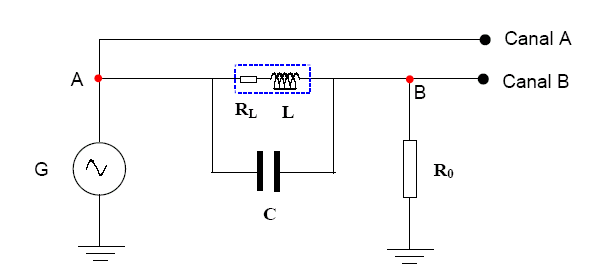
\includegraphics[width=9cm]{LG06--001.png}
    \caption{Esquema del circuito RLC paralelo.}
    \label{fig:circuitoRLCparalelo}
\end{figure}

En este circuito, la impedancia viene dada por la impedancia del paralelo $(L,C)$, que llamaremos $Z_{LC}$, en serie con la impedancia de la resistencia, $R$.
Dado que la inductancia tiene una resistencia interna $R_L$, tenemos 
\begin{equation}
    \frac{1}{Z_LC} = \frac{1}{Z_C} + \frac{1}{R_L+Z_L},
\end{equation}
es decir,
\begin{equation}
    Z_{LC} = \frac{ \left( R_L + j \omega L \right) \left( -\frac{j}{\omega C}  \right)   }{R_L + j \left( \omega L - \frac{1}{\omega C}\right)}.
\end{equation}
Para desfasaje nulo (\( \Delta \phi = 0\)), habrá un mínimo en la potencia transferida cuando la frecuencia angular sea igual a
\begin{equation}
    \omega_0' = \frac{1}{\sqrt{LC}} \sqrt{1 - R_L^2 \frac{C}{L}}.
\end{equation}
Observe que si la resistencia interna de la inductancia resulta nula, entonces
\begin{equation}
    \omega_0' = \frac{1}{\sqrt{LC}}.
\end{equation}


\subsection{Desarrollo de la experiencia}
Para esta segunda parte de la práctica, comience por montar el circuito de la figura \ref{fig:circuitoRLCserie}.
A continuación:
\begin{enumerate}
    \item Estudie la variación de la diferencia de potencial sobre la resistencia en función de la frecuencia de operación. 
    \item A partir de las mediciones realizadas en el inciso anterior, encuentre la frecuencia de antiresonancia y el valor de \(Q\).     
    \item Determine experimentalmente el desfasaje \( \Delta \phi(\omega)\) en función de la frecuencia; para lo cual puede resultarle útil el {\it modo XY} del osciloscopio.
    \item Compare los resultados de esta parte con aquellos obtenidos en el estudio del circuito RLC serie.
\end{enumerate}


\nocite{Alonso1998,Crawford1994,Purcell1988,Reitz1996,Trelles1984,Reitz1996}
\bibliographystyle{unsrt} 
\bibliography{Bibliografia}


\end{document}
